%%%%%%%%%%%%%%%%%%%%%%%%%%%%%%  IEEEsample.tex
%%%%%%%%%%%%%%%%%%%%%%%%%%%%%%%%%%%%%%%%%
%%%%%%%%%%%%%%%%%%%%%%%    More information: see the header of IEEEtran.sty
%%%%%%%%%%%%%%%%%%%%%%%
%%%%%%%%%%%%%%%%%%%%%%%%%%%%%%%%%%%%%%%%%%%%%%%%%%%%%%%%%%%%%%%%%%%%%%%%%%%%%%%%
%%%%

\documentclass{llncs}

\usepackage{helvet}
\usepackage{enumerate}
\usepackage{amsmath}
\usepackage{amsfonts}
\usepackage{graphicx}
\usepackage{multirow}
\usepackage{subfig}
\RequirePackage{algorithmic}
\RequirePackage{algorithm}


\input{epsf}
\def\BibTeX{{\rm B\kern-.05em{\sc i\kern-.025em b}\kern-.08em1
    T\kern-.1667em\lower.7ex\hbox{E}\kern-.125emX}}

%\newtheorem{Definition}{definition}[section]
%\newtheorem{example}{Example}
%\newtheorem{Lemma}{Lemma}

% New command for the table notes.
\def\tabnote#1{{\small{#1}}}

% New command for the line spacing.
\newcommand{\ls}[1]
    {\dimen0=\fontdimen6\the\font
     \lineskip=#1\dimen0
     \advance\lineskip.5\fontdimen5\the\font
     \advance\lineskip-\dimen0
     \lineskiplimit=.9\lineskip
     \baselineskip=\lineskip
     \advance\baselineskip\dimen0
     \normallineskip\lineskip
     \normallineskiplimit\lineskiplimit
     \normalbaselineskip\baselineskip
     \ignorespaces
    }

\newcommand{\beq}{\begin{equation}}
\newcommand{\eeq}{\end{equation}}
\newcommand{\ov}{\overline}
%\newcommand{\ov}{\bar}
\newcommand{\xor}{\bigoplus}
%%
%\newtheorem{algorithm}{Algorithm}[section]

\newcommand{\Fq}{{\mathbb{F}}_{q}}
\newcommand{\Fkk}{{\mathbb{F}}_{2^k}}
\newcommand{\Fkkx}[1][x]{\ensuremath{\mathbb{F}}_{2^k}[#1]\xspace}
\newcommand{\Grobner}{Gr\"{o}bner\xspace}
\newcommand{\B}{{\mathbb{B}}}
\newcommand{\F}{{\mathcal{F}}}
\newcommand{\G}{{\mathcal{G}}}
%%%

\newcommand{\debug}[1]{\textcolor{gray}{[ #1 ]}}


\begin{document}

\title{{Deriving Canonical Polynomial Representations from Circuits using Gr\"obner Bases}}

\author{
T. Pruss\inst{1} \and P. Kalla\inst{1} \and F. Enescu\inst{2}
}

\institute{
Electrical \& Computer Engineering\\
University of Utah, USA
\and
Mathematics \& Statistics\\
Georgia State University, USA
}

\maketitle

%\thispagestyle{empty}
%\pagestyle{empty}

\begin{center}{\bf ABSTRACT}\end{center}
Formal verification of hardware designs has become an essential
component of the overall system design flow. The designs are generally
modeled as finite state machines, on which property and equivalence
checking problems are solved for verification. Reachability analysis
forms the core of these techniques. However, increasing
size and complexity of the circuits causes the state explosion
problem. Abstraction is key to tackle the scalability challenge.

This dissertation presents new techniques for word-level abstraction
with applications in sequential design verification. By bundling
together $k$ bit-level state-variables into one word-level constraint 
expression, the state-space is construed as solutions (variety) to
a set of polynomial constraints (ideal), modeled over the finite
(Galois) field of $2^k$ elements. Subsequently, techniques from
algebraic geometry -- notably, Gr\"obner basis theory and technology
-- are researched to perform reachability analysis and
verification of sequential circuits. This approach adds a ``word-level
dimension'' to state-space abstraction and verification to make the
process more efficient.

While algebraic geometry provides powerful abstraction and reasoning
capabilities, the algorithms exhibit high computational complexity. In
the dissertation, we show that by analyzing the constraints, it is
possible to obtain more insights about the polynomial ideals, which can be
exploited to overcome the complexity. Using our algorithm design and
implementations, we demonstrate how to perform reachability
analysis of finite-state machines purely at the word-level. Using this
concept, we perform scalable verification of sequential arithmetic
circuits. As contemporary approaches make use of resolution proofs and
unsatisfiable cores for state-space abstraction, we introduce the
algebraic geometry analog of unsatisfiable cores, and present
algorithms to extract and refine unsatisfiable cores of polynomial
ideals. Experiments are performed to demonstrate the efficacy of our
approaches. 

\chapter{Introduction} \label{ch:intro}
There is an ever-increasing need for secure communication within information 
technology. Security of sensitive information relies more and more heavily 
on encryption methodologies implemented in hardware by cryptographic 
circuits. One of the most prominent of these methodologies is Elliptical 
Curve Cryptography (\emph{ECC}), which provides more strength per encryption bit 
than other encryption methodologies.
The main building blocks of ECC hardware implementations 
are fast, \emph{custom-built Galois field arithmetic circuits}.
These circuits are notoriously hard to verify, yet their correctness is 
vitally important in critical applications. In \cite{crypto:bug_attacks}, 
for example, it is shown that a bug in the hardware could lead to the full 
leakage of the secret cryptographic key, which could compromise the entire
system. Thus, formal verification is imperative in Electronic Design 
Automation (\emph{EDA}) when dealing with cryptographic circuits.

To facilitate this verification, it is highly desirable to obtain a {\it word-level 
representation of the datapath of the ECC arithmetic block} from its 
bit-level implementation. Ideally, this abstraction should be {\it canonical},
as this allows the it to be directly applicable to equivalence checking. 
Such a canonical, word-level abstraction of the 
Galois field arithmetic block would not only make it easier to verify and 
reason 
about the cryptographic system as a whole, but also enable the use of 
higher level abstraction and synthesis tools. 
As arithmetic circuits are custom-designed, often modularly, using Galois field arithmetic blocks, 
the abstraction should also exploit the hierarchical nature of the circuitry.
Due to the modular circuit structure, abstraction of each arithmetic block
becomes the key in verification of the full circuit. 
Practical 
applications of ECC dictate a datapath of a minimum of $163$-bits, up to 
$571$-bits, as 
designated by the National Institute for Standards and Technology (NIST).
However abstraction of 
Galois field arithmetic circuits has been infeasible for data-paths beyond 
$16$ bits. 

This dissertation proposes an algebraic geometry based approach to abstract canonical, 
word-level representations of bit-level Galois field arithmetic circuits.
The approach is able to abstract representations
for circuits up to 571 bits in size, which is the largest NIST
standard for datapath size in ECC. 
Verification of circuits for which this abstraction has been computed is shown to 
be trivial; thus, the focus is on deriving the abstraction quickly and efficiently.
%Furthermore, we show how we can use these abstract representations to 
%perform improved formal verification of these circuits.

\section{Hardware Design and Verification Overview}
The typical design flow of a hardware system, 
as shown in Fig. \ref{fig:cadflow}, starts with a hardware system 
specification, which describes the necessary functions and parameters that 
the system must perform and adhere to. The specification is typically
modelled using a transaction-level model (\emph{TLM}), which describes 
communication details between large circuit modules. 
The TLM is then translated 
into a register-transfer-level (\emph{RTL}) description, which is composed of abstracted, 
interconnected circuit blocks that compose the entire system. RTL is 
typically implemented 
in hardware description languages (\emph{HDL}) such as Verilog and VHDL, 
which are the most popular choices in the industry.
Next, the RTL is optimized and converted into a \emph{netlist}, i.e. a large 
collection of small physical blocks (MOSFET, Boolean logic gates, etc.) and 
the inter-connections (wires) between them. 
Lastly, the netlist is further optimized and then mapped onto a physical space 
on a chip, which is then sent off for fabrication. This entire design flow
is automated by Computer-Aided Design (\emph{CAD}) tools. 

{
\begin{figure}[h]
\centerline{
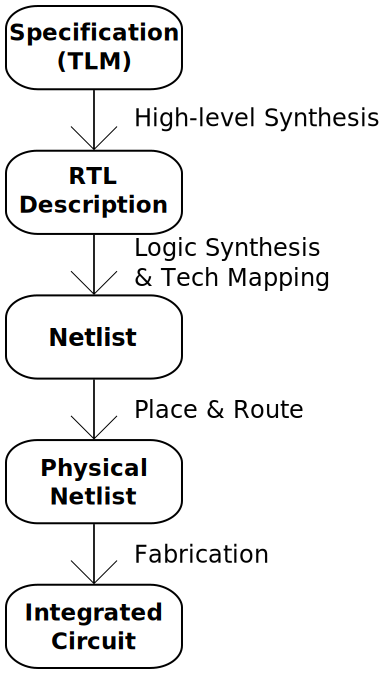
\includegraphics[width=0.5\textwidth]{./figures/designFlow}
}
\caption{Typical hardware design flow.}
\label{fig:cadflow}
\end{figure}
}

%\subsection{The Hardware Verification Imperative}
When moving from one abstraction level of the hardware design process to the 
next, an important issue arises: how can one ensure that the functionality of 
the optimized design matches original spec? 
Bugs in hardware design which are 
not caught early can have costly effects later, such as the need for a 
redesign. Bugs in arithmetic circuits can be especially catastrophic.
One infamous example is the 1994 floating point division (FDIV)
bug that affected the Intel Pentium chip \cite{nicely:FDIV}, 
and subsequently cost the company \$475 million because it was  
discovered after the chip's release. In another more fatal case, during the
Gulf war, an American Patriot Missile battery failed to intercept an incoming
enemy missile due to an arithmetic error \cite{arnold:patriot}.
Since hardware bugs can have significant consequences, 
there has been extensive work in field of hardware verification to find and
eliminate bugs prior to fabrication.

The two main methodologies used in hardware verification are simulation and 
formal verification. \emph{Simulation} checks correctness by applying exhaustive 
assignments to the circuit inputs and verifying correctness of the output. 
This ensures that the circuit performs as designed under all possible 
inputs. Such exhaustive testing is quite effective for smaller circuits. 
However, as the size of the circuit increases, it becomes 
computationally infeasible to simulate all possible test vectors. This is the 
case with Galois field arithmetic circuits, which are commonly very large in 
real-world applications. Often for such large circuits, simulations of a smaller and more 
manageable subset of test vectors are employed to catch bugs. While these tests
can increase confidence in the correctness of the design,  
{\it they do not guarantee correctness} since every data-flow of the design hasn't
been analyzed.
%Such is the case with large Galois field arithmetic circuits, so we instead 
%focus on formal verification. 

\section{Formal Verification}
Instead of simulating input vectors, \emph{formal verification} utilizes 
mathematical theory to reason about the correctness of hardware designs.
%which overcomes some limitations of simulation. 
Formal verification has two main forms: property checking and equivalence 
checking. 

{\it Property checking} (or property verification) verifies
that a design satisfies certain given properties. Property checking is done mainly 
in the form of theorem proving, model checking, or approaches which 
combine the two.
\begin{enumerate}
\item \emph{Theorem proving} \cite{theoremproving:91} requires the existence of
mathematical descriptors of the specification and implementation of the 
circuit. Theorem provers apply mathematical rules to these descriptors to
derive new properties of the specification. In this way, the tool can reduce
a proof goal to simpler sub-goals, which can be automatically verified.
However, generating the initial proof-goal requires extensive guidance from
the user, so there is an overall lack of automation in theorem 
proving.
\item \emph{Model checking} \cite{modelcheck:99} is an approach
to verifying finite-state systems where specification 
properties are modeled as a system of 
logic formulas. The design is then traversed to check if the 
properties hold. If the design is found to violate a
particular property, a counter-example is generated which exercises the
incorrect behavior in the design. Such counter-examples allow the designer
to trace the behavior and find where the error in the design lies.
Modern model checking techniques use the result to automatically refine
the system and perform further checking.
These tools are typically automated, and thus have found widespread 
use in CAD tool suites.
\end{enumerate}

{\it Equivalence Checking} verifies that two different representations of
a circuit design have equivalent functionality. An example of equivalence
checking as it applies to the hardware design flow is shown in
Fig. \ref{fig:equivflow}.

{
\begin{figure}[h]
\centerline{
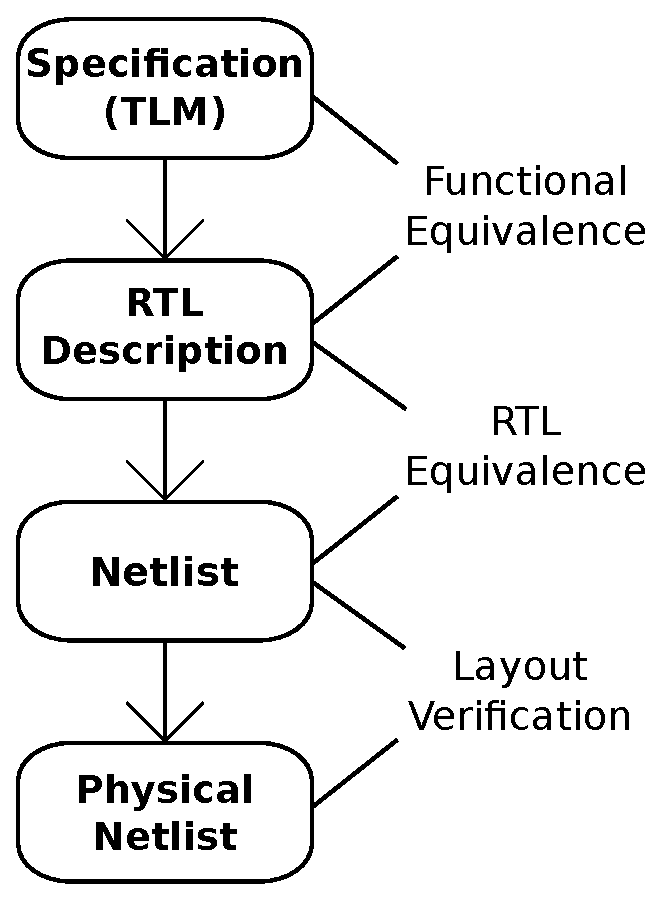
\includegraphics[width=0.5\textwidth]{./figures/designVerification}
}
\caption{Equivalence checking as applied to the hardware design flow.}
\label{fig:equivflow}
\end{figure}
}

There are two major
equivalence checking techniques: graph-based
and satisfiability-based.
\begin{enumerate}
\item \emph{Graph-based} techniques construct a canonical graph 
representation, such as a Binary Decision Diagram (\emph{BDD}) or one of
its many variants, of each circuit. A linear comparison is then conducted to 
determine whether the two graphs are isomorphic. Since the graph 
representation is canonical, the graphs of the two circuits will be 
equivalent if and only if the circuits perform the same function.
\item \emph{Satisfiability} techniques construct a miter of the two circuits,
typically in a graph such as an And-Inverter graph (\emph{AIG}). A
\emph{miter} is a combination of the two circuits with one bit-level output, which 
is only in a "1" state when the outputs of the circuits differ given 
the same given 
input, as shown in Fig. \ref{fig:miter}. 
A satisfiability (\emph{SAT}) tool \cite{csat} 
is then employed to simplify the graph and find a solution to the miter, 
i.e. find an input for which the 
miter output is "1". If a solution is found, this solution acts as a 
counter-example of when the circuit outputs differ; otherwise the circuits
are functionally equivalent.
\end{enumerate}


{
\begin{figure}[h]
\centerline{
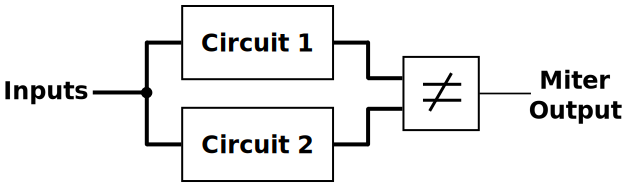
\includegraphics[width=0.8\textwidth]{./figures/betterMiter}
}
\caption{A miter of two circuits.}
\label{fig:miter}
\end{figure}
}

%\subsection{Computer-Algebra Based Formal Verification}
Certain formal verification methods use \emph{computer-algebra} and \emph{algebraic
geometry} techniques based on mathematical theories.
Unlike SAT-based verification, modern algebraic geometry 
techniques do not explicitly solve the constraints to find a solution; 
rather, they reason about the presence or absence of solutions, or explore
the geometry of the solutions.
These methods \cite{Avrunin:CAV} \cite{condrat-tacas07} \cite{gbverify:2007} 
transform the circuit design into a polynomial system. Typically, this system
of polynomials is then used to compute a Gr\"obner basis \cite{gb_book}. 
Computation of Gr\"obner bases allows for 
the easy deduction of important properties of a polynomial system, 
such as the presence or absence of 
solutions. These properties are then leveraged to perform 
verification. Unfortunately, such a computation 
has been shown to be doubly 
exponential in the worst case, and thus these methods have not been 
practical for real-world applications. However, recent
breakthroughs in computer-algebra hardware verification have shown
that it is possible to overcome the complexity of this computation while
still utilizing the beneficial properties of a Gr\"obner bases
\cite{lv:phd}.

\section{Importance of Word-level Abstraction}
Most formal verification techniques can benefit from word-level abstractions 
of the circuits they verify.
Abstraction is defined as state-space reduction, i.e{\text . }abstraction
reduces state-space by mapping the set of states of a system to a smaller 
set of states. Because the new representation contains fewer states, it
is easier to comprehend and thus easier to use. 
Word-level abstraction focuses specifically on abstracting a word-level
representation of a circuit out of a bit-level representation. For example,
a bit-level representation of an integer multiplier is represented by a
collection of Boolean inputs and outputs, whereas a word-level
abstraction hides the underlying logic and represents the circuit as two 
integer inputs and one integer output, e.g. $Z=A\cdot B$. As the bit-size of the
multiplier increases, the logical implementation of the multiplier grows (typically
exponentially) while the word-level abstraction stays the same.

Word-level abstractions have a wide variety applications in formal 
verification. Theorem proving techniques can leverage abstraction as an 
automatic decision procedure or as a canonical reduction 
engine. For example, since RTL is composed of circuit blocks that represent 
the underlying circuit, RTL verification methods can exploit 
abstractions of these blocks.
This is seen in the following RTL verification methods:
\begin{itemize}  
\item Model checking \cite{kroening:model}, 
where an approximation abstraction of RTL blocks is generated and then 
refined.
\item Graph-based equivalence 
checking \cite{WLS} \cite{arditi:bmd}, where abstraction methods are used
to generate a canonical word-level graph representation of the circuit.
\item Satisfiability-based equivalence checking \cite{lpsat}, where 
abstractions are used identify symmetrics and similarities in order to 
minimize the amount of logic that is sent to the 
SAT tool. 
\end{itemize}

Other equivalence checking techniques that employ abstractions 
include satisfiability modulo theory ({\it SMT}) techniques \cite{boolector} \cite{bryant:tacas07}, 
which are similar to SAT except they operate on higher-level data
structures (integers, reals, bit vectors, etc.), as well as 
constraint solving techniques \cite {ms:research} \cite{tew:iccad08}.
In general, RTL equivalence checking approaches would ideally maintain a 
high-level of abstraction while still retaining sufficient lower-level 
functional details  (such as bit-vector size, precision, etc) 
\cite{gupta_survey}.

Word-level hardware abstractions also have applications in RTL and datapath 
synthesis \cite{demicheli:iccad_98} \cite{demicheli:dac_99}
\cite{demicheli:tcad_03}. 
Abstractions of circuits allow for design reuse, which allows for tool-automated 
synthesis of larger circuit blocks.
Since hardware design specifications tend to be word-level, synthesis tools 
can use these larger circuit blocks to generate and optimize the
datapaths and create the RTL of the system. Thus, in order for a circuit to 
be used by these automated synthesis tools, its word-level abstraction must
be known.

Finally, abstractions can also be applied to detect malicious 
modifications to a circuit, potentially inserted as a hardware trojan horse.
Hardware trojans, a relatively new security concern in the hardware 
industry, use certain techniques to add incorrect behavior to a 
design. 
This behavior is only activated under certain rare circumstances that only 
the mal-intent designer has knowledge of.
The behavior is purposely hidden and is very difficult to encounter during 
simulation of the design. A manufactured chip with a subsystem 
that contains a hardware trojan could compromise the entire system in which 
it is used.
In some hardware trojan cases, formal verification techniques may be applied 
to catch a bug in a design and provide a counter-example which exercises it. 
However, it can be difficult to tell whether the bug in the design was 
introduced intentionally of not. On the other hand, word-level abstractions 
of bit-level circuits {\it effectively reverse-engineer the true function 
implemented by the circuit}, which could be used to determine the designer's 
true intention.

\section{Dissertation Objective, Motivation, and Contributions}
This dissertation focuses on abstracting a canonical, 
word-level representation of hardware (bit-level) implementations of 
combinational circuits. The proposed technique is a full abstraction solution which can be 
applied to any arbitrary acyclic combinational circuit. 
It is particularly efficient when applied to Galois field arithmetic circuits.
Using this technique, if the abstraction of the circuit's implementation and its
specification are found, they can be easily compared to determine equivalence.
Implementation of a custom software tool, developed to compute the abstractions, is
also described.

\subsection{Motivating Application}
The motivation for this work comes from applications of Galois field 
arithmetic circuits in elliptical curve cryptography ({\it ECC}) hardware systems.
The main operations of encryption, decryption, and 
authentication in ECC rely on operations performed on elliptic curves, which 
are implemented in hardware as polynomial functions over Galois fields. 
To be applicable in real-world situations, ECC data-paths
should be a minimum of $163$-bits wide, which is the minimum NIST standard, 
up to a recommended size of $571$-bit operand widths. Many non-ECC cryptosystems
have datapaths on the order of $1000$-bits.

A Galois field arithmetic circuit with a datapath size of $k$ 
is built as a Boolean function: $\mathbb{B}^k \rightarrow \mathbb{B}^k$. 
This function is mapped to an operation 
$f:\mathbb{F}_{2^k} \rightarrow \mathbb{F}_{2^k}$ 
over the Galois field $\mathbb{F}_{2^k}$. 
These circuits are custom-built, modular
systems which cannot be synthesized due to their complex nature. Thus, 
formal verification is needed to ensure they operate correctly.

Recent computer-algebra based formal verification techniques have been
able to perform verification of Galois field arithmetic circuits with
a datapath size up to $163$-bits \cite{lv:phd}. Word-level abstractions 
of Galois
field arithmetic circuits could be used to further improve these formal 
verification techniques to allow for verification of larger circuits, as
well as provide the other benefits of word-level abstraction.
However, there is currently no technique for computing word-level 
abstractions of Galois field circuits of any practical size.

{
\begin{figure}[h]
\centerline{
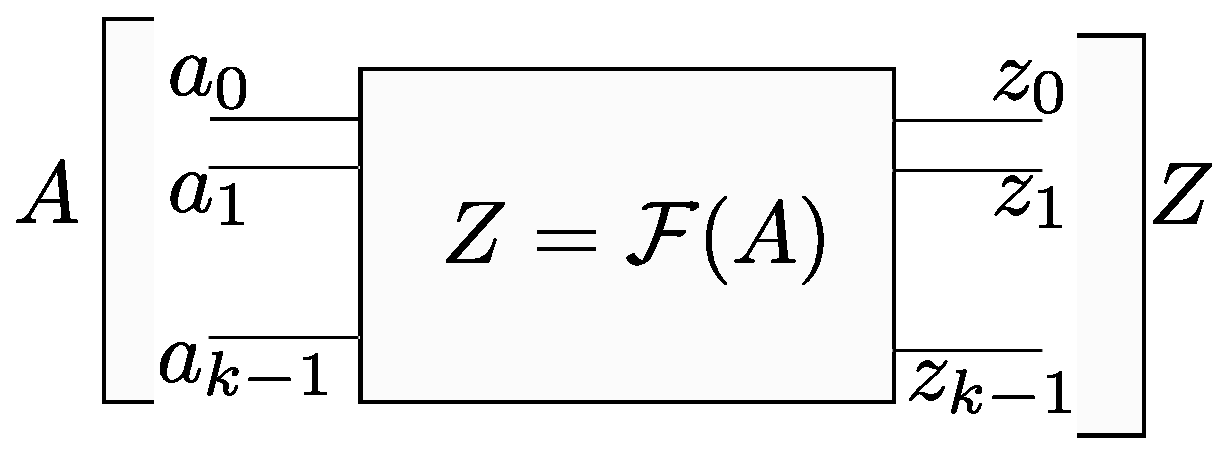
\includegraphics[width=0.5\textwidth]{./figures/interpolate}
}
\caption{Circuit with $k$-bit input $A$ and $k$-bit output $Z$. 
Abstraction to be derived as $Z=\Func(A)$.}
\label{fig:abstractA_Z}
\end{figure}
}

While the motivation comes from the need to verify Galois field arithmetic
circuits, the presented approach can be generalized to be applicable to any
combinational acyclic circuit.
Any such circuit with a $k$-bit input $A$ and a $k$-bit output $Z$, such
as the one shown in Fig. \ref{fig:abstractA_Z}, computes 
$f: \mathbb{B}^k \rightarrow \mathbb{B}^k$ and can thus be analyzed as the
function $f: \Fkk \rightarrow \Fkk$. Over $\Fkk$ this function can be 
represented as the polynomial $Z=\Func(A)$. This is trivially generalized
when there are multiple $k$-bit inputs $A_1,A_2,\dots,A_i$, i.e. $Z=\Func(A_1,\dots,A_i)$.
Now assume the word-size of the input differs from the output, that is the circuit
computes $f: \mathbb{B}^m \rightarrow \mathbb{B}^n$ for $m \neq n$. This can 
be represented as a function over Galois fields as $f: \F_{2^m} \rightarrow \F_{2^n}$.
This function can be analyzed over the field $\Fkk$ such that $\Fkk \supset \F_{2^m}$ 
and $\Fkk \supset \F_{2^m}$, where $k=LCM(m,n)$.

\subsection{Dissertation Contributions}
To solve the problem of word-level abstraction, this dissertation proposes 
a full solution consisting of three main contributions.

\begin{enumerate}
\item A theory for finding the word-level abstraction from a bit-level circuit over Galois fields is created.
The given bit-level circuit implementation is modelled as a system of
polynomials over the field.
This theory is derived using techniques from computer-algebra, notably the theory of
\Grobner basis \cite{pruss:iwls13}.
\item Using this theory, new algorithms based on symbolic computation are developed to 
derive the word-level abstraction. The algorithms are designed to be applicable to 
industry-size arithmetic circuits over Galois fields \cite{pruss:dac14}\cite{sun:date15}.
A complexity analysis of the algorithmic approach is also presented. Furthermore, the
approach is also generalized to make it applicable to arbitrary combinational circuits.
Finally, we show how the approach can be used to exploit the hierarchical structure of
large Galois field multipliers designed over composite fields.
\item A custom software tool implementation of the algorithmic approach is described, including
an analysis of efficient data structures designed for this purpose \cite{pruss:tcad15}.
\end{enumerate}

Experiments show that the proposed solution can abstract canonical, word-level, 
polynomial representations of Galois field arithmetic circuits up to $1024$-bits in
size, while other contemporary approaches are infeasible beyond a $32$-bit designs.


%an 
%approach based on computer-algebra, algebraic geometry - notably the theory of
%{\it Gr\"obner bases} \cite{gb_book} \cite{buchberger_thesis}.
%and {\it elimination ideals} \cite{ideals:book}, as our approach for 
%abstracting canonical word-level representations from bit-level Galois 
%field arithmetic circuits. 
%Computer-algebra techniques easily integrate with 
%Galois field theory and allow for polynomial abstraction of the circuit over 
%the field itself. Thus, if the circuit computes a function over some field $
%\mathbb{F}_{2^k}$, the resulting abstraction is a word-level polynomial 
%function over the same field $\mathbb{F}_{2^k}$. 

%The given bit-level circuit implementation is first modeled as a system of
%polynomials over the field. Using the theory of elimination ideals, we 
%derive an elimination term ordering and prove that by using this ordering we 
%can obtain a canonical word-level representation of a circuit by 
%computing a Gr\"obner basis of the polynomials. However, complexity 
%of the computation of a Gr\"obner basis proves to be prohibitive for circuits
%of practical size. Therefore, we employ a select sub-set of computations 
%from the Gr\"obner basis theory to overcome this complexity and obtain the
%abstraction. We prove that this simpler computation can be 
%performed via a polynomial reduction process, and engineer a custom 
%verification tool for this purpose. Using this approach, we are able to 
%successfully 
%abstract word-level representations of Galois field arithmetic circuits up 
%to $571$-bits, which is the {\it largest recommended NIST standard} for ECC.


\section{Dissertation Organization}
The rest of this dissertation is organized as follows. Chapter
\ref{ch:prev} reviews previous applicable work and highlights their
drawbacks with respect to the canonical, word-level abstraction problem. 
Chapter \ref{ch:prelim} describes the properties of Galois fields, 
$\mathbb{F}_{2^k}$, and explains the process of constructing them.
It also describes how to design arithmetic circuits over such fields, their 
complexities, and the role of these circuits in Elliptic Curve Cryptography.
Chapter \ref{ch:ideals} provides a theoretical background of 
computer-algebra and Gr\"obner bases and explains their application
to Galois fields. 
Chapter \ref{ch:abstract} describes an approach to abstract 
word-level polynomial representations of combinational circuits using a 
Gr\"obner basis computation.
Chapter \ref{ch:improv} improves on this word-level abstraction approach to 
make it applicable to much larger circuits.
Chapter \ref{ch:generalize} generalizes the abstraction approach to make
it applicable to circuits with varying operand word-lengths. It also describes how the 
approach can take advantage of the hierarchy of arithmetic circuits designed over
composite fields.
Chapter \ref{ch:implement} describes the implementation details of a 
custom abstraction tool and gives experimental results of
abstracting large Galois field multiplier circuits.
Chapter \ref{ch:concl} concludes the dissertation and outlines potential future 
research for continuation of this work. 

%% \section{Galois Fields, Polynomial Functions \& Hardware Design}
\label{sec:prelimgf}
%\vspace{-0.035in}

%% We briefly describe the relevant concepts related to Galois fields
%% $\Fkk$; for more details, interested readers may refer to the textbook 
%% \cite{galois_field:mceliece}. 
%% %to put the complexity of the verification problem in perspective, 
%% %to shed some light on the complexity of our design verification, 
%% We also review some VLSI architectures used for Galois field
%% computations \cite{mastro:phd} \cite{acar:1998} \cite{wu:2002}
%% \cite{Knezevic:2008} \cite{eccld} \cite{ecc163}. In our experiments,
%% we have verified custom designs based on these architectures. 

%%%%%%%%%%%%%%%%%%%%%%%%%%%%%%%%%%%%%%%%%%%%%%%%%%%%%%%%%%%%%%%%%%%%%%%%%%%%
%% %\begin{Definition}
%% A finite field, also called a {\bf Galois field}, denoted by $F_q$, is
%% a set of $q$ elements, including two distinguished elements 0 and 1,
%% along with operations $'+'$ and $'\cdot'$ (addition and
%% multiplication) that satisfy the following properties: 
%% \begin{itemize}
%% \item ($F_q, +, 0$) forms an Abelian group.

%% % \begin{itemize}
%% % \item  Closure: $\forall a, b \in F_q, a + b \in F_q$.
%% % \item Associativity: $\forall a, b, c \in F_q, a+(b+c)=(a+b)+c$.
%% % \item Commutativity: $\forall a, b \in F_q, a+b=b+a$.
%% % \item Additive Identity: $\forall a \in F_q, a+0=a$. 
%% % \item Additive Inverse: $\forall a \in F_q$, there is an additive
%% %   inverse element $-a \in F_q$ such that $a+(-a)=0$. 
%% %\end{itemize}

%% \item ($F_q, +, \cdot, 0, 1$) forms a commutative ring with unity.
%% % \begin{itemize}
%% % \item Multiplication closure: $\forall a, b \in F_q, a \cdot b \in
%% %   F_q$.
%% % \item Multiplication Associativity: $\forall a, b, c \in F_q, a \cdot
%% %   (b \cdot c)=(a \cdot b)\cdot c$.  
%% % \item Multiplication Commutativity: $\forall a, b \in F_q, a \cdot b=b \cdot a$. 
%% % \item Multiplication Identity: $\forall a \in F_q, a\cdot 1=a$. 
%% % \item Distributivity: $\forall a, b, c \in F_q, a \cdot (b+c)=(a
%% % \cdot b)+(a \cdot c)$. 
%% % \end{itemize}

%% \item Every non-zero element in $F_q$ has a   multiplicative inverse:
%%   $\forall a \in F_q - \{0\}, \exists a^{-1} \in F_q$ such that $a \cdot
%%   a^{-1}=1$. 

%% \item The number of elements $q$ of the finite field is a
%%   power of a prime integer, i.e. $q = p^k, k \geq 1, p=$ prime. 

%% \end{itemize}
%% %\end{Definition}

A Galois field is a field with a finite number of elements. The number
of elements $q$ of the field is a power of a prime integer --- i.e. $q
= p^k$, where $p$ is a prime integer, and $k \geq 1$ is a positive
integer \cite{galois_field:mceliece}. Galois fields are denoted as
${\mathbb{F}}_{q}$ and also $GF(q =p^k)$. We are interested in fields
where $p = 2$ and $k >1$ --- i.e. {\it   binary Galois extension
  fields} $\mathbb{F}_{2^k}$ --- as they are widely employed in
hardware implementations of cryptography primitives. 

To construct ${\mathbb{F}}_{2^k}$, we take the polynomial ring
${\mathbb{F}}_2[x]$, where ${\mathbb{F}}_{2} = \{0, 1\}$, and an
irreducible  polynomial $P(x) \in {\mathbb{F}}_2[x]$ of degree $k$, and
construct ${\mathbb{F}}_{2^k}$ as ${\mathbb{F}}_2[x] \pmod{   P(x)}$. As a
result, all field operations are performed 
modulo the irreducible polynomial $P(x)$ and the coefficients are
reduced modulo $p=2$. %=2$; due to which $-1 = +1$ over $\Fkk$. 
Any element $A \in {\mathbb{F}}_{2^k}$ can be represented in polynomial
form as $A = a_0 +  a_1 \alpha + \dots + a_{k-1} \alpha^{k-1}$, where
$a_i \in {\mathbb{F}}_2, i = 0, \dots, k-1$, and $\alpha$ is the root of
the irreducible polynomial, {\it i.e.} $P(\alpha)=0$. The field
$\Fkk$ can therefore be construed as a $k$-dimensional vector space
over ${\mathbb{F}}_2$.

%For
%example, $\mathbb{F}_{16} =  \mathbb{F}_2[x] \pmod{ x^4 + x + 1}$. 

%% \debug{
%% The {\it characteristic} of any finite field with
%% unity element $1$ is the least integer $n$ such that $1 + \dots + 1$
%% {\it (n times)} $= 0$. The characteristic of fields of the type
%% ${\mathbb{F}}_{p^k}$ %{\mathbb{F}}_p[x] \pmod{ P(x)}$ 
%% is the prime integer $p$. Since in our
%% case $p = 2$, all fields of the type $\Fkk$, for any given $k$, have 
%% characteristic 2. As a result, all field operations are performed
%% modulo the irreducible polynomial $P(x)$ and the coefficients are
%% reduced modulo $p=2$; due to which $-1 = +1$ over $\Fkk$. 
%% }

%% Any element $A \in \mathbb{F}_{2^k}$ can be represented in polynomial
%% form as $A = a_0 +  a_1 \alpha + \dots + a_{k-1} \alpha^{k-1}$, where
%% $a_i \in \mathbb{F}_2, i = 0, \dots, k-1$, and $\alpha$ is the root of
%% the irreducible polynomial, {\it i.e.} $P(\alpha)=0$. The field
%% $\Fkk$ can therefore be construed as a $k$-dimensional vector space
%% over $\mathbb{F}_2$.



\begin{Example}\label{ex:1}
Let us construct ${\mathbb{F}}_{2^4}$ as ${\mathbb{F}}_2[x] \pmod{
  P(x)}$, where $P(x)=x^4+x^3+1 \in {\mathbb{F}}_2[x]$ is an
irreducible polynomial of degree $k =4$. Let $\alpha$ be the root of
$P(x)$, i.e. $P(\alpha)=0$.  Any element $A \in {\mathbb{F}}_2[x]
\pmod{ x^4 + x^3 + 1}$ has a representation of the type: $A = a_3 x^3
+ a_2 x^2 +  a_1 x + a_0$ where the coefficients $a_3, \dots, a_0$ are
in ${\mathbb{F}}_2 = \{0, 1\}$. Since there are only 16 such
polynomials, we obtain 16 elements in the field
${\mathbb{F}}_{16}$. Each element in can then be viewed as a 4-bit
vector over ${\mathbb{F}}_2$: ${\mathbb{F}}_{16}=\{(0000),(0001),
\dots (1110),(1111)\}$.  Each element also has an exponential
representation; all three representations are shown in Table
\ref{tab:gfelement}. For example, consider the element $\alpha^{12}$.
Computing $\alpha^{12} \pmod{ \alpha^4+\alpha^3+1} = \alpha + 1
= (0011)$; hence we have the three equivalent representations. 

\vspace{-0.1in}
\begin{table}[h]
\begin{center}
{\small
\caption{Bit-vector, Exponential and Polynomial representation of
elements in  ${\mathbb{F}}_{2^4} = {\mathbb{F}}_2[x]
\pmod{x^4+x^3+1}$}\label{tab:gfelement}  
\begin{tabular}{|c|c|c||c|c|c|} 
\hline
$a_3a_2a_1a_0$ & Exponential & Polynomial     &$a_3a_2a_1a_0$ & Exponential & Polynomial  \\
\hline
$0000$        & $0$         & $0$            & $1000$ & $\alpha^3$ &  $\alpha^3$\\
\hline
$0001$        & $1$         & $1$            & $1001$ & $\alpha^4$ & $\alpha^3 + 1$\\
\hline
$0010$        & $\alpha$    & $\alpha$       & $1010$ & $\alpha^{10}$&$\alpha^3 + \alpha$  \\
\hline
$0011$        & $\alpha^{12}$& $\alpha + 1$   & $1011$ & $\alpha^5$ & $\alpha^3+\alpha+1$\\
\hline
$0100$        & $\alpha^2$  & $\alpha^2$     &  $1100$ & $\alpha^{14}$ & $\alpha^3 + \alpha^2$\\
\hline
$0101$        & $\alpha^9$   &$\alpha^2 + 1$ & $1101$  &$\alpha^{11}$  & $\alpha^3+\alpha^2+1$\\
\hline
$0110$        & $\alpha^{13}$& $\alpha^2 + \alpha$ & $1110$ & $\alpha^8$& $\alpha^3+\alpha^2+\alpha$\\
\hline
$0111$        &$\alpha^7 $ & $\alpha^2+\alpha+1$ & $1111$ &$\alpha^6$ & $\alpha^3+\alpha^2+\alpha+1$\\
\hline
\end{tabular}
}
\end{center}
\end{table}
\end{Example}




%%%%%%%%%
{\bf Polynomial Functions $f: \Fkk \rightarrow \Fkk$:} 
Arbitrary mappings among $k$-bit vectors can be constructed; each such
mapping generates a function $f: \B^k \rightarrow \B^k$. Since every
$k$-bit vector can be construed as an element in $\Fkk$ (as shown in
the above example), every such function corresponds to a function over
Galois fields: $f: \Fkk \rightarrow \Fkk$. Every such function is also
a polynomial function. 

\begin{Theorem}
From \cite{ff:1997}: 
Let $\Fq$ be a Galois field of $q$ elements where $q$ is a power of a
prime integer. Any  function $f: \Fq \to \Fq$ is a polynomial function
over $\Fq$, that is there exists a polynomial $\F \in \Fq [x]$ such
  that $f(a) = \F(a)$, for all $a \in \Fq$. 
\end{Theorem}

By analyzing $f$ over each of the $q$ points, one can apply
{\bf Langrange's interpolation formula} and interpolate a polynomial
$\F(x) = \sum_{k=1} ^q  \frac{ \prod_{i \neq k}  (x -x_i)}{\prod_{i \neq k}
  (x_k -x_i)} \cdot f(x_k)$, which is a polynomial of degree at 
most $q-1$ in $x$. One can easily see that $\F(a)=f(a)$ for all $a \in
\Fq$, and $\F(x)$ is therefore the polynomial function representation
of $f$. 

\begin{Example} {\it
Let $A = \{a_2, a_1, a_0\}$ and $Y = \{y_2, y_1,
y_0\}$ be 3-bit vectors.  Consider the function $Y[2:0] = A[2:0]
>> 1$, i.e. a {\bf bit-vector right shift} operation on $A$. 
The function maps as follows:

\begin{center}
{\small
\begin{tabular}{c|ccc|c||c|ccc|c}
$\{a_2a_1a_0\}$  & $A$ &$\rightarrow$& $\{y_2y_1y_0\}$ &$Y$ &
  $\{a_2a_1a_0\}$  &$A$&$\rightarrow$& $\{y_2y_1y_0\}$ &$Y$\\
\hline
000  &0 &$\rightarrow$& 000 & 0 & 100  &$\alpha^2$ &$\rightarrow$& 010 &  $\alpha$ \\
001  &1 &$\rightarrow$& 000 & 0 & 101  &$\alpha^2 + 1$ &$\rightarrow$&010 & $\alpha$ \\
010  &$\alpha$ & $\rightarrow$ & 001& 1 & 110  &$\alpha^2 + \alpha$&$\rightarrow$& 011 &$\alpha + 1$ \\   
011  &$\alpha + 1$ &$\rightarrow$& 001 &1 & 111& $\alpha^2 + \alpha + 1$ &$\rightarrow$& 011 &$\alpha + 1$\\
\hline
\end {tabular}
}
\end{center}

If we model this function as $f: {\mathbb{Z}}_{8} \rightarrow
{\mathbb{Z}}_{8}$, then using the results of \cite{singmaster}
\cite{chen_95} \cite{chen_96}, we deduce that this function is not a
polynomial function over ${\mathbb{Z}}_{8}$. However, applying
Largange's interpolation formula over ${\mathbb{F}}_{2^3}$, we obtain
the following polynomial function representation, $Y =
(\alpha^2+1)A^4+(\alpha^2+1)A^2$, where $P(\alpha) = \alpha^3 +
\alpha + 1 = 0$. 
}
\end{Example}

An important property of Galois fields is that for all elements $A \in
{\mathbb{F}}_q, A^q = A$, and hence $A^q - A =  0.$ Therefore, the
polynomial $x^q -x$ {\it vanishes} on all points in
$\Fq$. Consequently, any polynomial $\F(X)$ can be reduced $\pmod{ X^q
  - X}$ to obtain a canonical representation $\F(X) \pmod{X^q - X}$
with degree at most $q-1$. Such {\it vanishing polynomials} will form
an important part of our ideal membership formulation.  


\begin{Definition}
Any function $f: \Fq^d \to \Fq$ has a unique canonical representation
(UCR) as polynomial $\F \in \Fq[x_1,\dots, x_d]$ such that all its 
nonzero monomials are of the form $x_1^{i_1}\cdots x_d^{i_d}$ where $0
\leq i_j \leq q-1$, for all $j=1, \ldots d$.
\end{Definition}


\subsection{Hardware Implementations of Galois Field Arithmetic}
% Operations Over $\mathbb{F}_{2^k}$}

{\bf Point Addition over Elliptic Curves:} The main operations of
encryption, decryption and authentication in elliptic curve
cryptography (ECC) rely on {\it point additions} and {\it doubling}
operations on elliptic curves designed over Galois fields. 
%Point multiplication involves a series of addition and doubling of
%points on the elliptic curve. % -- this, in turn, requires finite
%field multiplications.  
%A drawback of traditional approaches is that they require
%point multiplication is that each point addition and doubling 
In general, this requires computation of multiplicative inverses over
the field - which is expensive. Modern approaches represent
the points in projective coordinate systems, {\it e.g.}, the
L$\acute{o}$pez-Dahab (LD) projective coordinate \cite{eccld},
%\cite{ecc:software},
which eliminates the need for multiplicative inverses and improves the
efficiency of these operations. 

%%%

%% \begin{Example}
%% {\it 
%% Consider point addition in L$\acute{o}$pez-Dahab (LD) projective
%% coordinate. Given an elliptic curve: $Y^2 + XYZ = X^3Z + aX^2Z^2 +
%% bZ^4$ over $\mathbb{F}_{2^k}$,   where $X,Y,Z$ are $k$-bit vectors
%% that are elements in $\mathbb{F}_{2^k}$ and similarly, $a, b$ are
%% constants from the field.   Let ($X_3$, $Y_3$, $Z_3$) = ($X_1$, $Y_1$,
%% $Z_1$) + ($X_2$, $Y_2$, $1$)  represent point addition over the
%% elliptic curve.  Then $X_3$, $Y_3$, $Z_3$ can be computed as follows: 

%% \begin{align*}
%% A &= Y_2 \cdot Z_1^2 + Y_1 \\
%% B &= X_2 \cdot Z_1 + X_1 \\
%% C &= Z_1 \cdot B \\
%% D &= B^2 \cdot(C + a Z_1^2) \\
%% Z_3 &= C^2 \\
%% E &= A \cdot C  \\
%% X_3 &= A^2 + D + E  \\
%% F &= X_3 + X_2 \cdot Z_3 \\
%% G &= X_3 + Y_2\cdot Z_3 \\
%% Y_3 &= E\cdot F + Z_3 \cdot G \\
%% \end{align*}
%% }
%% \end{Example}

\begin{Example}
{\it 
Consider point doubling in LD projective coordinate system. Given an
elliptic curve: $Y^2 + XYZ = X^3Z + aX^2Z^2 + bZ^4$.  
Let  ($X_3$, $Y_3$, $Z_3$) = 2($X_1$, $Y_1$, $Z_1$), then $X_3, Y_3,
Z_3$ can be computed as: $X_3 = X_1^4 + b \cdot Z_1^4; ~~Z_3 = X_1^2
\cdot Z_1^2; ~~Y_3 = b Z_1^4 \cdot Z_3 + X_3 \cdot (aZ_3 + Y_1^2 +
bZ_1^4 )$. 
}
\end{Example}

The multiplication and iterative squaring operations in the above
computation are usually implemented using custom-designed Galois field
multipliers, such as the Mastrovito \cite{mastro:1989}, Montgomery
\cite{acar:1998}, Barrett multipliers \cite{Knezevic:2008}, or
composite-field multipliers \cite{cfmulti:1996} --- which are, in
turn, hierarchically designed.  For example, Montgomery reduction (MR)
computes: $MR(A,B)=A\cdot B \cdot R^{-1} \pmod {P(x)}$, 
where $A,B$ are $k$-bit inputs, $R$ is suitably chosen as
$R={\alpha}^k$, $R^{-1}$ is multiplicative inverse of $R$ in
${\mathbb{F}}_{2^k}$, and $P(x)$ is the irreducible polynomial.
Since Montgomery reduction cannot directly compute $A\cdot B \pmod
{P(x)}$, we need to pre-compute $A\cdot R$ and $B\cdot R$, as shown in
Figure \ref{fig:mm4}.   

\begin{figure}[hbt]
	\begin{center}
	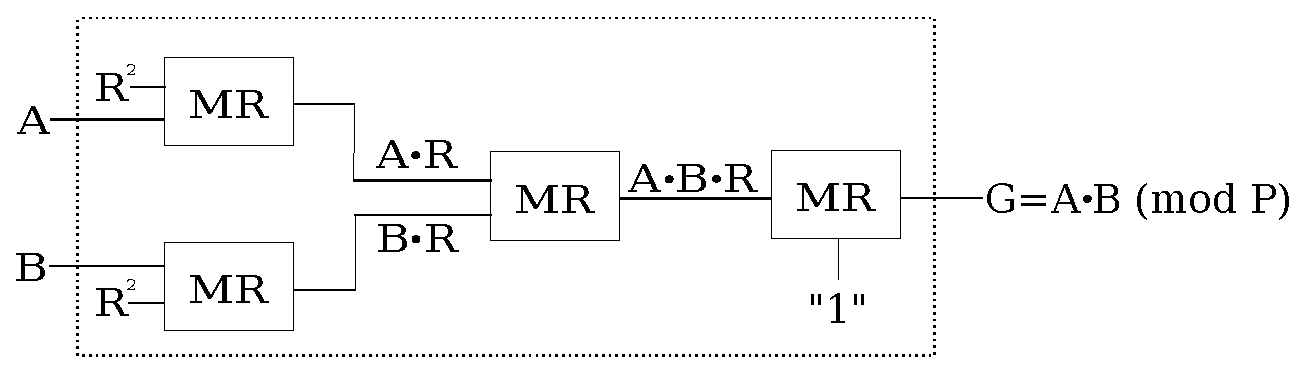
\includegraphics[scale=0.4]{new_mmcircuit.eps}
	\end{center}
	\caption{{\it Montgomery} multiplication over $\mathbb{F}_{2^k}$
          using four Montgomery reductions.}
	\label{fig:mm4}
\end{figure}

Given a hierarchically designed Montgomery multiplier, we will first
extract polynomials $AR, BR, ABR$ from the sub-circuit blocks. By
analyzing the interconnection of these sub-circuits at word-level, we
can then apply our approach at a higher-level, to extract the function
of the entire circuit. Performing such operations hierarchically, we
will apply our approach to reverse-engineer point-addition circuits
designed using a variety of such Galois field adder and multiplier
circuits.  

%% \input{setup}
%% %\input{promodel}
%% %\input{solve}
%% \section{Experiment results}
We have implemented our core extraction approach (the GB-Core
algorithm) using the \textsc{Singular} symbolic
algebra computation system [v. 3-1-6] \cite{DGPS}. With our
tool implementation, we have performed experiments to extract a
minimal unsat core from a given set of  
polynomials. Our experiments run on a desktop with
3.5GHz Intel $\text{Core}^\text{TM}$ i7-4770K Quad-core CPU, 16 GB RAM and
64-bit Ubuntu Linux OS.

%Nowadays most SAT benchmarks are huge, which choke our GB engine. 
Gr\"obner basis is not an efficient engine for solving contemporary
CNF-SAT benchmarks that are of large size. In order to validate our
approach, we use a customized  benchmark library: "aim-100" is revised
from ramdon 3-SAT benchmark "aim-50/100", "subset" series are generated for
random subset sum problems, "cocktail" is revised from a mixed
factorization/random 3-SAT benchmark, and "phole4/5" are generated by
adding redundandant clauses to pigeon hole benchmarks. Moreover, we
created SMPO/RH benchmarks that correspond to
equivalence checking instances of sequential Galois field normal basis
modulo multiplier implementations (also known as Agnew's multiplier \cite{SMPO}
and Reyhani-Hassan multiplier \cite{RHmulti} respectively) against the golden model spec. 
Similarly, the "MasVMon" benchmarks are the miter circuits of
 Mastrovito multipliers compared against  Montgomery
multipliers. The CNF formulae are translated as polynomial constraints
over $\mathbb{F}_2$ (as shown in \cite{condrat-tacas07}), and the
GB-Core algorithm is applied. 
%These benchmarks are in moderate size for our GB engine but not too trivial. 

\vspace{-0.1in}
\begin{table}[htb]
\centering
\caption{\centering Results of running benchmarks using our tool\\
\small{Asterisk($^*$) denotes a benchmark which is not converted from CNF benchmark}}
\begin{tabular}{|c||c|c|c|c|c|c|}
\hline
\multirow{4}{2.2cm}{\centering Benchmark} 
& \multirow{4}{0.9cm}{\centering \# Polys} 
& \multirow{4}{0.8cm}{\centering \# MUS} 
& \multirow{4}{1.9cm}{\centering Size of core w/ iterative refinement heuristic}
 & \multirow{4}{1.6cm}{\centering \# GB-core iterations}
 & \multirow{4}{2cm}{\centering \# Size of core after using syzygy heuristic}
 & \multirow{4}{1.3cm}{\centering Runtime (sec)} \\
  & & & & & & \\
    & & & & & & \\
      & & & & & & \\
\hline
\hline
$5\times 5$ SMPO & 240  & 137  & 137  & 8  &  & 3160\\
$4\times 4$ SMPO$^*$ & 84  & 21  & 21  & 1  &  & 125\\
$3\times 3$ SMPO$^*$ & 45  & 15  & 15  & 1  &  & 6.6\\
$3 \times 3$ SMPO & 17 & 2 & 2 & 1 &  & 0.07  \\
$4 \times 4$ MasVMont$^*$ & 148 & 83 & 83 & 1 &  & 23 \\
$3 \times 3$ MasVMont$^*$ & 84 & 53 & 53 & 1 &  & 4.3 \\
$2 \times 2$ MasVMont & 27 & 23 & 23 & 2 &  & 2.3 \\
$5\times 5$ RH$^*$ & 142  & 34  & 35  & 4  &  & 1001\\
$4\times 4$ RH$^*$ & 104  & 35  & 36  & 3  &  & 98\\
$3\times 3$ RH$^*$ & 50  & 20  & 20  & 1  &  & 2.9\\
aim-100 & 79 & 22 & 22 & 1  &  & 43\\
cocktail & 135 & 4 & 4 & 2 &  & 5 \\
subset-1 & 100 & 6 & 6 & 1 &  & 2.4 \\
subset-2 & 141 & 19 & 23 & 2 & 21 & 12 \\
subset-3 & 118 & 16 & 12 & 2 & 11 & 8.7 \\
phole4 & 104 & 10 & 16 & 1 & 10 & 4.4 \\
phole5 & 169 & 19 & 25 & 3 & 19 & 14 \\
\hline
\end{tabular}
\label{tab:result}  
\end{table} 

In Table \ref{tab:result}, we list the details of our experimental
results. In the table, \#Polys denotes the given number of polynomials
from which a core is to be extracted. \#MUS is the minimal core
extracted by PicoMUS. \#GB-core iterations corresponds to the
number of calling GB-core engine to arrive at an unsatisfiable core. The
second last column is showing the improvement of minimal core
size applying syzygy heuristic on cases which are not able to be
refined further with the iterative heuristic.
The data shows that in most of these
cases, our tool can produce a minimal core when our iterations
converge. From the experimental results we can also make the
observation that the GB-core algorithm, particularly Theorem
\ref{thm}, offers quite a lot of scope for identifying redundant
polynomials that can be eliminated from the core --- without resorting
to a brute-force membership check of every polynomial $f_i \in F -
\{f_i\}$. 




\section{Conclusions}
This paper addressed the problem of identifying an infeasible core of
a set of multivariate polynomials, with coefficients from a field,
that have no common zeros. The problem is posed in the context of
computational algebraic geometry and solved using the Gr\"obner basis
algorithm. We show that by recording the data produced by the
Buchberger's algorithm -- the $Spoly(f_i,f_j)$ pairs, as well as the
polynomials of $F$ used in the division process
$Spoly(f_i,f_j)\xrightarrow{F}_+ 1$ -- we can identify certain
conditions under which a polynomial can be discarded from a core. An
algorithm was implemented within the Singular computer algebra tool
and some experiments were conducted to validate the approach. While
the use of GB engines for SAT solving has a rich history, the problem
of unsat core identification hasn't been fully addressed by the SAT
community. We hope that this paper will kindle some interest in this
topic which is worthy of attention from the SAT community. 

%% %\input{conclusion}


%%%%%%%%%%%%%%%%%%%% The bibliography %%%%%%%%%%%%%%%%%%%%%%%%%%%%
\bibliographystyle{splncs03}
%\bibliographystyle{/Users/Kalla/tex/inputs/ieee}
\bibliography{logic,oldlogic}
\end{document} 




